\chapter*{Kurzfassung der Diplomarbeit/Abstract} \addcontentsline{toc}{chapter}{Kurzfassung der Diplomarbeit/Abstract}



\newlength{\htllogobreite}
\htllogobreite29mm
\newlength{\beschriftungsbreite}
\beschriftungsbreite127mm
\newlength{\feldA}
\feldA50mm
\newlength{\feldB}
\feldB77mm

\begin{tabular}{|p{\htllogobreite}|p{\beschriftungsbreite}|}
\hline
\multirow{2}{\htllogobreite}{\epsfig{figure=images/htl_logo_beschnitten.eps, width=29mm, angle=0}}&{\vspace{0.05em}\textbf{HÖHERE TECHNISCHE LEHRANSTALT YBBS AN DER DONAU}}\\[1.05em]
\cline{2-2}
 & { \begin{tabular}{p{\feldA} p{\feldB}}
    Fachrichtung:&\textbf{Informationstechnologie}\\
    Ausbildungsschwerpunkte:&\textbf{Netzwerktechnik}\\
   \end{tabular}
   }\\
\hline
\end{tabular}

\begin{center}
 \LARGE \textbf{DIPLOMARBEIT}\\
 \Large \textbf{DOKUMENTATION}\\
 \normalsize
\end{center}

\newlength{\feldC}
\feldC49mm
\newlength{\feldD}
\feldD107mm

\linespread{1.1} \normalsize
\begin{tabular}{|p{\feldC}|p{\feldD}|}
 \hline
 Namen der Verfasser/innen & David Pöchacker, Marcel Entner, Tobias Kronsteiner \\
 \hline
 Jahrgang Schuljahr & 5AHITN  2021/22 \\
 \hline
 Thema der Diplomarbeit &Echtzeit Visualisierung von Energiesystemen \\
 \hline
 Kooperationspartner & Bioenergy and Sustainable Technologies GmbH\\
 \hline
\end{tabular}

\begin{tabular}{|p{\feldC}|p{\feldD}|}
 \hline
 Aufgabenstellung & Das Ziel der Diplomarbeit \grqq Echtzeit Visualisierung von Energiesystemen\glqq \space ist, dem Unternehmen Best GmbH eine zentrale Verwaltung von Energiesystemen bereitzustellen. Zusätzlich zur Verwaltung soll es möglich sein, Echtzeitdaten von einer ausgewählten Energietechnologie in Form von Statistiken zu visualisieren.\\
 \hline
\end{tabular}

\begin{tabular}{|p{\feldC}|p{\feldD}|}
 \hline
 Realisierung & Die Weboberfläche wurde mit Laravel umgesetzt. Eingegebene Daten werden in einer Datenbank erfasst und mittels Grafana auf der \\&Weboberfläche visualisiert. Abrufbar ist das Produkt über eine vom Auftraggeber bereitgestellte Domain mit dazugehörigem Webserver.  \\
 \hline
\end{tabular}

\begin{tabular}{|p{\feldC}|p{\feldD}|}
 \hline
 Ergebnisse &  Mithilfe des Produkts können Energiesysteme sowie Energietechnologien erstellt, bearbeitet und gelöscht werden. Ein rollenbasiertes Benutzersystem regelt den Zugriff auf die Verwaltung der einzelnen Energiesysteme. Der Administrator hat als Einziger die Möglichkeit neue Benutzer hinzuzufügen oder bestehende zu löschen. Jedem Benutzer ist es möglich, die Grafana Statistiken seiner selbst erstellen Energietechnologien anzeigen zu lassen.\\
 \hline
\end{tabular}

\begin{tabular}{|p{\feldC}|p{\feldD}|}
 \hline
 Architektur &   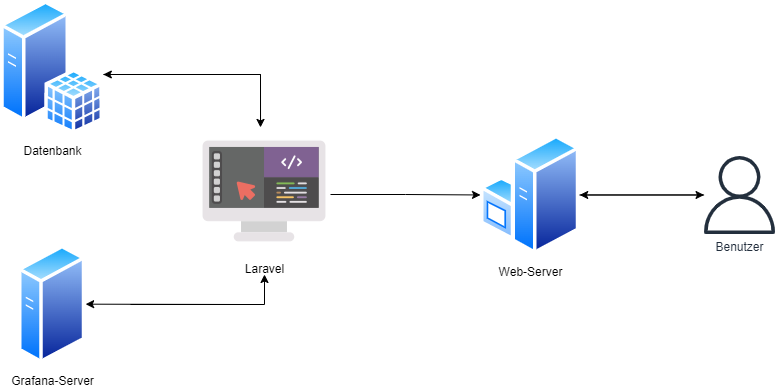
\includegraphics[height=4cm]{images/Architektur}\\ 
 
 
 \hline
\end{tabular}


\begin{tabular}{|p{\feldC}|p{\feldD}|}
 \hline
 Teilnahme an Wettbewerben, & Mostviertler Schulinovationspreis \\
 Auszeichnungen & noch keine\\
 \hline
\end{tabular}

\begin{tabular}{|p{\feldC}|p{\feldD}|}
 \hline
 Möglichkeiten der Einsicht- & Bibliothek des SZ-Ybbs \\
 nahme in die Arbeit & \\
 \hline
\end{tabular}

\newlength{\feldE}
\feldE51mm


\begin{tabular}{|p{\feldC}|p{\feldE}|p{\feldE}|}
 \hline
 Approbation \small{Prüfer}& \scriptsize{Prüfer/Prüferin} & \scriptsize{Direktor bzw. Abteilungsvorstand}\\ 
 (Datum / Unterschrift)& & \\
 \hline
\end{tabular}
\linespread{1.25} \normalsize

\clearpage

% Makro um in vorgegebener Spaltenbreite zentrieren zu können
\newcolumntype{C}[1]{>{\centering\arraybackslash}m{#1}}

\begin{tabular}{|p{\htllogobreite}|C{\beschriftungsbreite}|}
\hline
\multirow{2} {\htllogobreite} {\epsfig{figure=images/htl_logo_beschnitten.eps, width=29mm, angle=0}} & \vspace{0.05em}\textbf{HÖHERE TECHNISCHE LEHRANSTALT YBBS AN DER DONAU}\\
& \textbf{COLLEGE of ENGINEERING}\\[0.05em]
\cline{2-2}
 & { \begin{tabular}{p{\feldA} p{\feldB}}
    Department:&\textbf{Information Technology}\\
    Educational focus:&\textbf{Network and Media Technology}\\
   \end{tabular}
   }\\
\hline
\end{tabular}

\begin{center}
 \LARGE \textbf{DIPLOMA THESIS}\\
 \Large \textbf{Documentation}\\
 \normalsize
\end{center}

\linespread{1.1} \normalsize
\begin{tabular}{|p{\feldC}|p{\feldD}|}
 \hline
 Author(s) & David Pöchacker, Marcel Entner, Tobias Kronsteiner \\
 \hline
 Form & \\ Academic year & 5AHITN  2021/22\\
 \hline
 Topic & Echtzeit Visualisierung von Energiesystemen\\
 \hline
 Co-operation Partners & Bioenergy and Sustainable Technologies GmbH\\
 \hline
\end{tabular}

\begin{tabular}{|p{\feldC}|p{\feldD}|}
 \hline
 Assignment of Tasks & The goal of the diploma thesis \grqq Echtzeit Visualisierung von Energiesystemen\glqq \space is to provide the company Best GmbH with a central management of energy systems. In addition to the administration it should be possible to visualize real-time data from a selected energy technology in the form of statistics.\\
 \hline
\end{tabular}

\begin{tabular}{|p{\feldC}|p{\feldD}|}
 \hline
 Realisation &  The web interface was implemented with Laravel. Data is entered into a database and visualized on the web interface using Grafana. The product can be accessed via a domain provided by the Best GmbH with an associated web server. \\
 \hline
\end{tabular}

\begin{tabular}{|p{\feldC}|p{\feldD}|}
 \hline
 Results & With the product, energy systems as well as energy technologies can be created, edited and deleted. A role-based user system regulates access to the administration of the individual energy systems. The administrator is the only one who has the possibility to add new users or delete existing ones. Each user is able to view the Grafana statistics of his self-created energy technologies. \\
 \hline
\end{tabular}

\begin{tabular}{|p{\feldC}|p{\feldD}|}
 \hline
 Architecture &  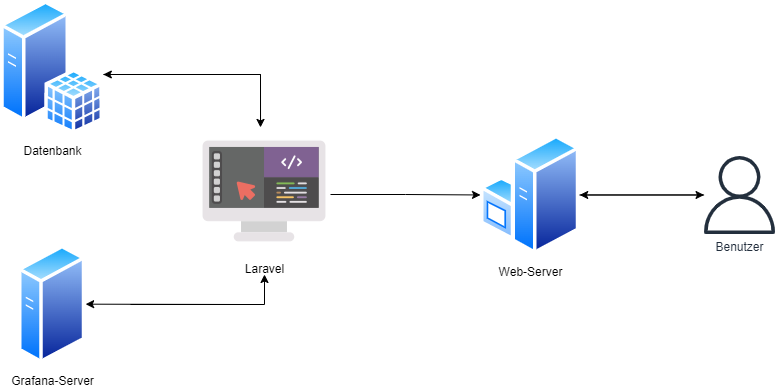
\includegraphics[height=4cm]{images/Architektur}\\
 \hline
\end{tabular}

\begin{tabular}{|p{\feldC}|p{\feldD}|}
 \hline
 Participation in Competitons &  Mostviertler Schulinovationspreis\\
 Awards & not yet awarded\\
 \hline
\end{tabular}

\begin{tabular}{|p{\feldC}|p{\feldD}|}
 \hline
 Accessibility of Diploma Thesis & Library of the SZ-Ybbs\\
 \hline
\end{tabular}

\begin{tabular}{|p{\feldC}|p{\feldE}|p{\feldE}|}
 \hline
 Approval & \scriptsize{Examiner} & \scriptsize{Head of College / Department}\\ 
 (Date / Sign)& & \\
 \hline
\end{tabular}
\linespread{1.25} \normalsize
